\chapter{Development}
\label{ch.development}

		\todo[inline]{Need a better introducion. vvvv--- this is only copy-paste from proposal.}

	The proposal for this undergraduate dissertation is made up of two main contributions.
	The first contribution will be the port of the \textit{Inter-Cluster Communication Module},
	described in \autoref{sec.inter-cluster-communication}, for the \mppa manycore processor.
	The second contribution will be the design and implementation of communication services
	of a master-slave \os, described in \autoref{sec.communication-services}, on top of
	the inter-cluster communication module.

		\todo[inline]{Insert some paragraphs about the development, tools, etc.}

	\section{Low-Level Communication}
	\label{sec.low-level-comm}
	\todo{Or: Nanvix HAL Level}

		O Nanvix HAL provê o módulo de comunicação inter-cluster para permitir que cluster distintos troquem informações.
		Esse módulo é constituido de três abstrações, nomeados Sync, mailbox e portal.
		Essas abstrações proveêm mecânismos mais precisos, fáceis de usar, escalonáveis e facilmente portáveis para diferentes arquiteturas~\cite{wentzlaff_fleets:_2011}.
		Sobre eles, é possível criar dos mais simples serviços, como sincronização e troca de dados, à serviços mais complexos como \shm, POSIX Semaphore, \rmem~\cite{penna:rmen}.
		O comportamento esperado pode ser simulado por ambos tipos de chamadas, sincronas ou assíncronas, dependendo apenas do suporte em hardware.
		Motivados a expor melhor controle sobre QoS para as camadas superiores, nós dissociamos as pequenas transferência de dados das grandes, isto é, mailbox e portal.
		Vale notar que seria possível utilizar uma NoC para cada abstração se o hardware suportasse.
		Não fizemos isso no MPPA porque a CNoC só provê a transferência de valores de 64 bits.

		FALAR DAS MOTIVAÇOES E DECISÕES QUE LEVARAM A ESCOLHA DAS 3 ABSTRAÇÕES

		Está seção está organizada da seguinte maneira.
		Subseção 0 abrange pontos comuns entre todas as abstrações.
		Subseção 1, 2 e 3 apresentam conceitualmente cada uma das abstrações, os problemas que elas englobam, e detalhes de implementação.

		\subsection{\mppa Hardware Resources}
		\label{sec.mppa-hardware-resources}

			A realização da comunicação de baixo-nível depende principalmente de dois recursos do MPPA, interrupções e DMA.
			Primeiro, o sistema de interrupções permitirá a configuração de tratadores das mensagens recebidas e enviadas através da NoC.
			Isto possibilitará a assíncronidade das operações, ponto vital em um sistema operacional baseado no microkernel onde o mestre não pode ficar bloqueado esperando a conclusão de uma única comunicação.
			Caso não fosse possível realizar pelo menos a recebimento de dados/sinais de forma assíncrona, sérios problemas de desempenho seriam introduzidos as camadas superiores.
			Segundo, o DMA é o mediador de todas as comunicações, síncrona ou assíncronas.
			Neste ponto, um hypervisor virtualiza a DMA, separando-a em duas estruturas lógicas globais, uma para a CNoC e outra para a DNoC.
			Cada estrutura agrupa os registradores para a configuração de envio/recebimento, e campos de bits indicando quais slots geraram uma interrupção.
			O hypervisor executa nos RM e controla, de forma assíncrona, as permissões de leitura/escrita dos registradores virtualizados.

			O controle efetuado pelo hypervisor não engloba a alocação ou manipulação dos recursos.
			Consequentemente, nós controlamos manualmente a alocação através de campos de bits.
			Caso uma operação não esteja em conformidade com esse controle, é retornado um valor negativo indicando o erro, \eg alocação de um recursos que já está em uso.
			Assim, não inflingimos custos indesejados ao transferir a responsabilidade de tratar o erro a camada superior, \eg aguardar a liberação do recurso.
			A manipulação envolve procedimentos para configurar a DMA com as devidas permissões e garantir a coerência de cache das operações.
			Por fim, vale ressaltar que não é realizado nenhum controle de concorrência sobre as estruturas comentadas para que não seja inflingido um sobre custo sobre a abordagem do microkernel.
			Caso a HAL seja utilizada para desenvolver um sistema operacional monolítico, o mesmo deve se preocupar em garantir a atômicidade das operações.

			A DMA coordena três linhas de interrupções.
			Duas delas são utilizados pela DNoC para notificar o recebimento de dados e o término do envio dados por uma microthread.
			A CNoC só utiliza uma linha para o recebimento de sinais porque o envio de um sinal, um valor de 64-bits, é realizado explicitamente pelo core.
			Para cada linha de interrupção existe um handler específico mas todos executam um algoritmo similar.
			O Algoritmo 3 exemplifica de forma simplificada o comportamento de um handler.
			Devido ao fato que a linha apenas notifica qual o tipo de interrupção, é responsabilidade do manipulador varrer os recursos de cada interface procurando quem acionou a interrupção.
			Para que não ocorresse a perda de interrupções, foi garantido que o manipulador fosse reentrante.
			Devido ao abordagem do microkernel, os problemas de concorrência são amenizados porque apenas o mestre trata as interrupções.

			\begin{algorithm}
				\caption{Simplified NoC Handler Algorithm.}%
				\label{alg.noc-handler}%
				\begin{algorithmic}[1]
					\Require $status[M_{Interfaces}][N_{Resources}]$, interrupt status of a resource.
					\Require $handlers[M_{Interfaces}][N_{Resources}]$, interrupt handler of a resource.
					\Procedure{noc\_handler}{}
					\For {$i \in [1, M_{Interfaces}]$}
						\For {$j \in [1, N_{Resources}]$}
							\If {$status[i][j] == Interrupt Triggered$}
								\State {$\Call{clean\_status}{i, j}$}
								\State {$\Call{handlers[i][j]}{i, j}$}
							\EndIf
						\EndFor
					\EndFor
					\EndProcedure
				\end{algorithmic}%
				\fonte{Developed by the Author.}%
			\end{algorithm}

			NoC interfaces have two identifiers, one physical (physical ID) and the other logical (logical ID).
			The hardware uses the physical IDs in the process of data routing through \noc.
			Each physical ID is associated with a Logical ID to enable the identification
			of \noc nodes outside the \hal.
			Logical IDs primarily serve to disassociate the node identification from the
			architecture that implements the \hal.
				\autoref{tab.noc-node-id} shows the physical and logical identification performed for \mppa.
			A Tabela 3 apresenta o mapeamento proposto para os clusters do MPPA.
			Cada linha apresenta um dos três grupos de nós NoC existentes (primeira coluna), agrupados por proximidade dos identificadores lógicos.
			Dentro de cada grupo temos um conjunto de identificadores físicos (segunda coluna) que são mapeados 1 para 1 para os identificadores lógicos (terceira coluna).
			Por exemplo, o grupo IO0 constitui 4 interfaces, onde são mapeadas da seguinte forma: $128 \to 0$, $129 \to 1$, $130 \to 2$, e $131 \to 4$.
			A ordem do mapeamento foi definido desta maneira para ficar mais intuitivo qual das interfaces, por consequência o cluster, é o mestre.
			Neste caso, o nó mestre é o identificador lógico 0, IO0.
			Este processo facilita na sincronização após o boot.

			\begin{table}[!tb]
				\centering%
				\caption{NoC Interface Identification.}%
				\label{tab.noc-node-id}%

				\begin{tabular}{l|l|l|}
					\cline{2-3}
															& \textbf{Physical ID} & \textbf{Logical ID} \\ \hline
					\multicolumn{1}{|l|}{\textbf{\iocluster0}} & 128-131              & 0-3                 \\ \hline
					\multicolumn{1}{|l|}{\textbf{\iocluster1}} & 192-195              & 4-7                 \\ \hline
					\multicolumn{1}{|l|}{\textbf{\ccluster}}   & 0-15                 & 8-23                \\ \hline
				\end{tabular}

				\fonte{Developed by the Author.}%
			\end{table}

			Para performar a comunicação entre dois clusters, é necessário que o emissor conheça qual o identificador do recurso que o receptor irá usar.
			Por exemplo, caso o receptor configurar o recebimento em um recurso da DNoC e o emissor enviar para outro, mesmo que o identificador lógico esteja correto, o receptor não será notificado do recebimento.
			Por esta razão, os slots de recebimento da CNoC e DNoC foram particionados por abstração.
			Dentro de uma partição, cada slot é mapeado estaticamente para um identificador lógico, \eg 0 à 23.
			Em contraste, os canais de envio não possuem essa necessidade, podendo ser alocados dinâmicamente.
			Entretanto, um conceito importante do Nanvix HAL é prover os recursos necessários para uma determinada operação sem realizar otimizações desnecessárias.
			Desta forma, os canais de envio também foram particionados por abstração de modo que sejam reservados durando toda uma operação.
			A tabela 3 apresenta cada abstração, identificados pelas linhas, e o particionamento dos recursos de cada NoC, identificados pelas colunas.
			Como a abstração sync não realiza a troca de dados arbitrários, não foram reservados recursos na DNoC.
			Vale notar que mesmo com a não utilização de todos os slots existentes, o aperfeiçoamento da programabilidade por não necessitar especificar os recursos de uma comunicação é um ponto forte do design das abstrações.

			% To perform the communication between two clusters, it is necessary that the
			% sender knows which resource the receiver will use.
			% For this reason, the receive slot range of \cnoc and \dnoc are partitioned
			% by abstraction, as can be seen in \autoref{tab.noc-resources}.
			% Within a partition, each slot is associated with a cluster's logical ID.
			% 	\todo{"On the another hand" does not make sense AGAIN.}
			% On the other hand, the transmitters use sending channels that need to
			% be reserved during the entire operation.
			% 	\todo{Explain the table.}
			% Thus, \autoref{tab.noc-resources} also shows the partition of the
			% sending channels for each abstraction.

			\begin{table}[!tb]
				\centering%
				\caption{Partitions of NoC resources by abstraction.}%
				\label{tab.noc-resources}%

				\todo[inline]{Explicar a motivação na separação dos recursos. Por que o portal tem 2 cnoc tx?}

				\begin{tabular}{l|l|l|l|l|}
					\cline{2-5}
															& \multicolumn{2}{c|}{\textbf{\cnoc}}          & \multicolumn{2}{c|}{\textbf{\dnoc}}          \\ \cline{2-5}
															& \textbf{RX Slot ID} & \textbf{TX Channel ID} & \textbf{RX Slot ID} & \textbf{TX Channel ID} \\ \hline
					\multicolumn{1}{|l|}{\textbf{\mailbox}} & 0-23                & 0                      & 0-23                & 1-3                    \\ \hline
					\multicolumn{1}{|l|}{\textbf{\portal}}  & 24-47               & 1-2                    & 24-47               & 4-7                    \\ \hline
					\multicolumn{1}{|l|}{\textbf{\sync}}    & 48-71               & 3                      & -                   & -                      \\ \hline
				\end{tabular}

				\fonte{Developed by the Author.}%
			\end{table}

			Por fim, nós conseguimos remover quase toda dependência com a pilha de software disponibilizada pela Kalray.
			Porém, ao eliminar as biliotecas de comunicação, a falta de documentação da virtualização do hardware e exemplos funcionais de comunicação, surgiram limitações no envio dos dados pela DNoC.
			Resumidamente, não foi possível configurar corretamente as microthreads existentes na DMA para envio assíncrono, tornando-se um trabalho futuro.
			Entretanto, tal limitação não impactou no design das abstrações exigindo apenas que o core mestre perca um tempo enviando os dados manualmente.

		\subsection{General Concepts of Communication Abstractions}
		\label{sec.general-concepts}

			Tecnicamente, o Nanvix HAL não sabe que tipos de aplicações ou kernels o utilizaram.
			Desta forma, é preciso garantir um comportamento comum que não afete o funcionanto da camada superior.
			O microkernel, especificamente, restringe o core mestre a estar quase sempre disponível para atender solicitações dos escravos.
			Por isso, as interfaces exportam apenas chamadas assíncronas (isto é, funções async e wait).
			Isto força a camada superior, caso queira, criar chamadas síncronas que chamam a função wait logo após a operação assíncrona.
			Deste modo, no nível do microkernel, nós conseguimos garantir que o mestre configure ou execute as funções assíncronas e notifique os escravos que aguardam na função wait.
			No MPPA, este controle é realizado através de spinlocks atrelados a cada recurso das abstrações.
			Ao concluir uma operação, o mestre libera o bloqueio para o escravo continuar sua execução.

			Contudo, a limitação da DMA descrita na Seção 0 acrescenta um agravante na operação de transferência das abstrações mailbox e portal.
			Nestas abstrações, existe um controle de fluxo onde o receptor deve notificar o emissor, dando-lhe permissão para transferir os dados.
			Este comportamento pode ocasionar o bloqueio do mestre ao esperar uma permissão.
			Para burlar esse problema, foi introduzido o conceito de envio preguiçoso.
			O algoritmo 4 ilustra o comportamento do envio preguiçoso, onde o mestre guarda os paramêtros caso não tenha permissão e vai atender outras solicitações.
			Ao receber a permissão do receptor, o manipulador de interrupções identifica o recurso, realiza de fato o envio dos dados e libera o escravo que solicitou o envio.
			Assim, nós garantimos que o mestre deixe de fazer algo útil e trave todo o sistema.

			\begin{algorithm}
				\caption{Simplified Lazy Transfer Algorithm.}%
				\label{euclid}%
				\begin{algorithmic}[1]
				\Require $resources$, Abstraction Resource Table

				\Algphase{Configures data transfer.}

					\Procedure{async\_write}{$id, message, size$}
						\State {$resources[id].message \gets message$}
						\State {$resources[id].size \gets size$}
						\If {$resources[id].has\_permission$} 
							\State {$\Call{do\_lazy\_write}{id}$}
						\Else
							\State {$resources[id].is\_waiting \gets True$}
						\EndIf
					\EndProcedure%

				\Algphase{Receives permission.}

					\Procedure{abstraction\_handler}{$id$} 
						\If {$resources[id].is\_waiting$} 
							\State {$\Call{do\_lazy\_write}{id}$} 
						\Else
							\State {$resources[id].has\_permission \gets True$}
						\EndIf
					\EndProcedure%

				\Algphase{Transfers the data.}

					\Procedure{do\_lazy\_write}{$id$} 
						\State {$resources[id].is\_waiting \gets False$}
						\State {$resources[id].has\_permission \gets False$}
						\State {$\Call{transfer\_data}{resources[id].message, resources[id].size}$} 
						\State {$\Call{unlock}{resources[id].lock}$}                                \Comment{Releases slave core.}
					\EndProcedure%

				\end{algorithmic}%

				\fonte{Developed by the Author.}%
			\end{algorithm}

			Por fim, as interfaces das abstrações seguem uma convenção para distinguir os papeis de receptor e emissor.
			Receptores utilizam as funções com sufíxo \texttt{create}, \texttt{unlink}, \texttt{aread} e \texttt{wait}.
			Emissores, por sua vez, utilizam funções com sufíxo \texttt{open}, \texttt{close}, \texttt{awrite} e \texttt{wait}.
			Como a função \texttt{wait} é compartilhada, a abstração deve fazer a distinção do papel pelo identificador do recurso.
			A diferenciação da natureza das operações ajuda tanto o usuário, sendo bastante intuitivo, como na implementação da HAL por explicitar quais recursos serão necessário.

			% Por fim, como já comentado anteriormente, o Nanvix HAL não realiza nenhum tipo de multiplexação dos recursos físicos do hardware.
			% A quantidade de recursos de comunicação disponíveis é diretamente relativa a quantidade de recursos físico para realizar uma dada operação.
			% A tabela 4 mostra quais recursos físicos são necessário para cada abstração e a quantidade total de abstrações simultaneas que podem existir.
			% Por exemplo, a criação de um portal precisa de um slot de recebimento da DNoC e 1 canal de transmissão da CNoC.
			% As quantidades são baixas devido aos poucos canais de transmissão, porém quem deve se preocupar com a multiplexação dos recursos deve ser da camada superior.

			% \begin{table}[!tb]
			% 	\centering%
			% 	\caption{Physical requirements by abstraction.}%
			% 	\label{tab.abstractions-amount}%

			% 	\begin{tabular}{l|l|l|l|l|l|l|}
			% 		\cline{2-7}
			% 												& \multicolumn{3}{c|}{\textbf{Create}}  & \multicolumn{3}{c|}{\textbf{Open}}                              \\ \cline{2-7}
			% 												& \multicolumn{1}{|c|}{\textbf{RX}}
			% 												            & \multicolumn{1}{|c|}{\textbf{TX}}
			% 															            & \multicolumn{1}{|c|}{\textbf{Available}}
			% 																		                & \multicolumn{1}{|c|}{\textbf{RX}}
			% 																				                    & \multicolumn{1}{|c|}{\textbf{TX}}
			% 																				        			            & \multicolumn{1}{|c|}{\textbf{Available}} \\ \hline
			% 		\multicolumn{1}{|l|}{\textbf{\mailbox}} & 1 (\dnoc) & 1 (\cnoc) & 1             & 1 (\cnoc) & 1 (\dnoc) & 4                                        \\ \hline
			% 		\multicolumn{1}{|l|}{\textbf{\portal}}  & 1 (\dnoc) & 1 (\cnoc) & 2             & 1 (\cnoc) & 1 (\dnoc) & 4                                        \\ \hline
			% 		\multicolumn{1}{|l|}{\textbf{\sync}}    & 1 (\cnoc) & 0         & 24            & 0         & 1 (\cnoc) & 1                                        \\ \hline
			% 	\end{tabular}

			% 	\fonte{Developed by the Author.}%
			% \end{table}

		\subsection{Sync Abstraction}
		\label{sec.sync-abs}

			A abstração de sincronização, chamada sync, provê o básico para a sincronização de clusters.
			A partir dela, é possível criar barreiras distribuidas.
			Seu comportamento é análogo a abstração POSIX Signals, mas as notificações não carregam informações, servem apenas para sincronização.
			O sync define dois modos de sincronização, ALLTOONE e ONETOALL.
			Nois dois modos, os clusters são separados entre um único nó mestre (ONE) e um ou mais nós escravos (ALL).
			A Figura 1 ilustra o modo ALLTOONE, onde o nó mestre aguarda bloqueado os N escravos realizarem a sincronização.
			Em contrapartida, o modo ONETOALL é utilizado quando o mestre notifica os N escravos, liberando-os do bloqueio, ilustrado pela Figura 3.
			Os nós emissores nunca ficam bloqueados, o trabalho deles é emitir um sinal.
			Os nós receptores são responsáveis por aguardar a chegada de todas as notificações.

			\begin{figure}[!tb]
				\centering%
				\caption{Synchronization Abstraction Example.}%
				\label{fig:sync-concepts}%

				\subcaptionminipage[fig:sync-all-to-one]%
					{.6\linewidth}%
					{N Slaves notify the Master (\texttt{ALL\_TO\_ONE}).}%
					{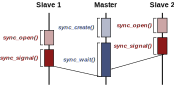
\includegraphics[width=\linewidth]{sync-all-to-one.pdf}}%
				\hfill
				\subcaptionminipage[fig:sync-one-to-all]%
					{.6\linewidth}%
					{The Master notify N Slaves (\texttt{ONE\_TO\_ALL}).}%
					{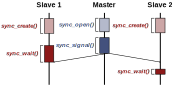
\includegraphics[width=\linewidth]{sync-one-to-all.pdf}}%

				\fonte{Developed by the Author.}%
			\end{figure}

			\subsubsection{Receiver Side Implementation}

% O que é a interface?
% Quais são os parâmetros para realizar uma operação?
				O Codigo 4 apresenta a interface Sync para nós receptores proposta para o Nanvix HAL.
				Os parâmetros necessário para a abertura de um ponto de sincronização é uma lista de IDs lógicos, o tamanho da lista e o tipo de sincronização.
				A lista deve ser sempre inicializada com o ID do nó mestre, independentemente do modo.
				Os identificadores restantes, contando que não tenham repetição, podem estar em qualquer ordem.
				O tipos de sincronização são os modos descritos anteriormente definidos através de constantes.
				As demais funções utilizam o identificador da abstração retornado pela função de criação.
				Caso algum parâmetro esteja em desacordo ou inválido, um valor negativo é retornado indicando o erro, \eg, \texttt{nodes == NULL}.

\begin{listing}[!tb]
\caption{Nanvix HAL: Sync Interface for Receiver Node.}
\label{code:hal-sync-receiver}
\begin{minted}{c}
/**
 * @brief Allocates and configures the receiving side of
 * the synchronization point.
 */
int sync_create(const int *nodes, int nnodes, int type);

/* @brief Releases and cleans receiver slot. */
int sync_unlink(int syncid);

/* @brief Waits a signal. */
int sync_wait(int syncid);
\end{minted}
\fonte{Developed by the Author.}
\end{listing}

% Quais recursos são necessário para cada tipo de operação, envio e recebimento?
				O recebimento das notificações requer a reserva 1 slot rx da CNoC relativo ao identificador do mestre.
				Deste modo, eliminamos o conflito no uso de diferentes slots por diferentes configurações de sincronização.
				Em contrapartida, um nó não poderá ser o mestre em duas operações simultâneas.
				O total de abstrações que podem ser criadas desta maneira é igual a quantidade de nós existentes (24 no MPPA).
				Nos cluster I/O, este total é multiplicado pelo número de interface NoC disponíveis, ou seja, 24 por DMA.
				A configuração do slot é realizado através de uma máscara de 64-bits.
				Está mascará é construida com os IDs lógicos dos emissores de modo que os bits relativos a suas posições sejam iguais a 0.
				Ao receber um sinal, a DMA realiza um OR com o valor anterior.
				Quando todos os bits se tornarem 1's, a DMA zera todos os bits do registrador e emite uma interrupção.

% Como as operações funcionam?
				Um vetor de estruturas internas realiza o controle das operações.
				Cada posição do vetor é reservado a um slot físico e guarda flags de controle, a mascará e um spinlock.
				Ao realizar a abertura, espera ou unlink de um sync, a HAL verifica discrepâncias nos IDs, nas flags de controle ou nos parâmetros.
				Por fim, o spinlock é utilizado para sincronização da operação com os núcleos escravos.
				Em um sistema microkernel, o core mestre configura o sync e o escravo aguarda ser liberado no spinlock.
				O tratador de interrupções do Sync identifica a estrutura e libera o bloqueio.
				A falta de coerência de cache não afeta os spinlock porque são utilizadas instruções que garantem a atomicidade que implementam o lock.

% Como foi resolvido o problema de multiplos nós nos IOs? PRECISA FALAR? DARIA PRA ARRUMAR ISSO NO CÓDIGO FORÇANDO QUE O ID[1] FOSSE O ID LOCAL (CASO NAO FOR O MESTRE).
				% A lista de nós foi projetada para utilizar os IDs das interfaces NoCs ao invés dos IDs dos Cluster para não desperdiçar as DMAs extras existentes nos Cluster I/O.

			\subsubsection{Sender Side Implementation}

% O que é a interface?
% Quais são os parâmetros para realizar uma operação?
				A interface do nó emissor, apresentada pelo Código 3, utiliza os mesmo parâmetros para abertura de um sync.
				Ao utilizar os mesmo valores na criação e abertura, a aplicação cliente pode definir o papel do cluster simplemente definindo qual função deve ser chamada.
				Entretanto, tanto na criação quanto na abertura, o ID lógico local deve estar Range correto do lista.
				Por exemplo, um sync é aberto com o ID local como mestre mas o tipo de sincronização é definido como ALL\_TO\_ONE.
				Isto retornará um erro e o sync não será aberto porque o mestre deveria ser o receptor das notificações e não o emissor.
				O restante da implementação segue o que já foi explicado na seção anterior.

\begin{listing}[!tb]
\caption{Nanvix HAL: Sync Interface for Sender Node.}
\label{code:hal-sync-sender}
\begin{minted}{c}
/**
 * @brief Allocates and configures the sending side of
 * the synchronization point.
 */
int sync_open(const int *nodes, int nnodes, int type);

/* @brief Releases the transfer channel. */
int sync_close(int syncid);

/* @brief Sends a signal. */
int sync_signal(int syncid);
\end{minted}
\fonte{Developed by the Author.}
\end{listing}

% Quais recursos são necessário para cada tipo de operação, envio e recebimento?
				De maneira oposta ao receptor, o emissor necessita de 1 canal de envio da CNoC para abrir um sync.
				Devido a separação dos canais descritos na seção (MPPA HARDWARE), um nó só poderá abrir um sync por vez.
% Como as operações funcionam?
				Para emitir um sinal, o nó precisa identificar o ID lógico e o slot de recebimento do mestre.
				A mascará que será ser enviada é sempre um valor de 64-bits com o bit relativo ao nó emissor setado como 1.
				A estrutura de controle do emissor também possui flags para garantir a semântica das operações.
				Somado a isso, o emissor guarda, em um array de inteiros, todos os IDs lógicos dos destinatário do sinal.
				Ao performar de fato o envio, será configurado e enviado um sinal para cada target desta lista.
				O envio do sinal é realizado através da escrita em um registrador da DMA, desta maneira, não é possível realizar esta ação de forma assíncrona como as demais abstrações.

		\subsection{Mailbox Abstraction}
		\label{sec.mailbox-abs}


			% The \textit{Mailbox Abstraction} allows clusters to exchange fixed-size
			% messages with each other.
			% The message was thought to be a relatively small size, usually a few hundred bytes.
			% Similarly, the operation of the \mailbox follows \posix message queue behavior.
			% For example, the message can be used to encode small operations and system
			% control signals.
			% As illustrated in \autoref{fig:conpt_mailbox}, the operation cardinality is N:1,
			% where N senders can transfer one message at a time to a receiver queue.
			% When the receiver consumes a message, it notifies the sender to ensure
			% control of the flow.

			A abstração \textit{Mailbox} permite que clusters troquem mensagens
			de tamanho fixo entre si.
			O tamanho da mensagem foi projetado para ser relativamente pequeno,
			geralmente algumas centenas de bytes.
			Essas mensagens são consumidas pelo receptor sem a necessidade de conhecer quem as enviou.
			A Figura (conceito) ilustra conceitualmente uma das formas de implementar uma Mailbox.
			O receptor aloca espaço suficiente para receber 1 mensagem de cada possível emissor.
			O emissor envia para o espaço reservado para sua mensagem, eliminando a concorrência de escrita das mensagens.
			Similarmente, a operação da \mailbox segue o comportamento da fila de mensagens \posix.

			\begin{figure}[!tb]
				\centering%
				\caption{Mailbox Abstraction Concept.}%
				\label{fig:conpt_mailbox}%

				\subcaptionminipage[fig:conpt_mailbox-logical]%
					{.5\linewidth}%
					{Conceptual Overview.}%
					{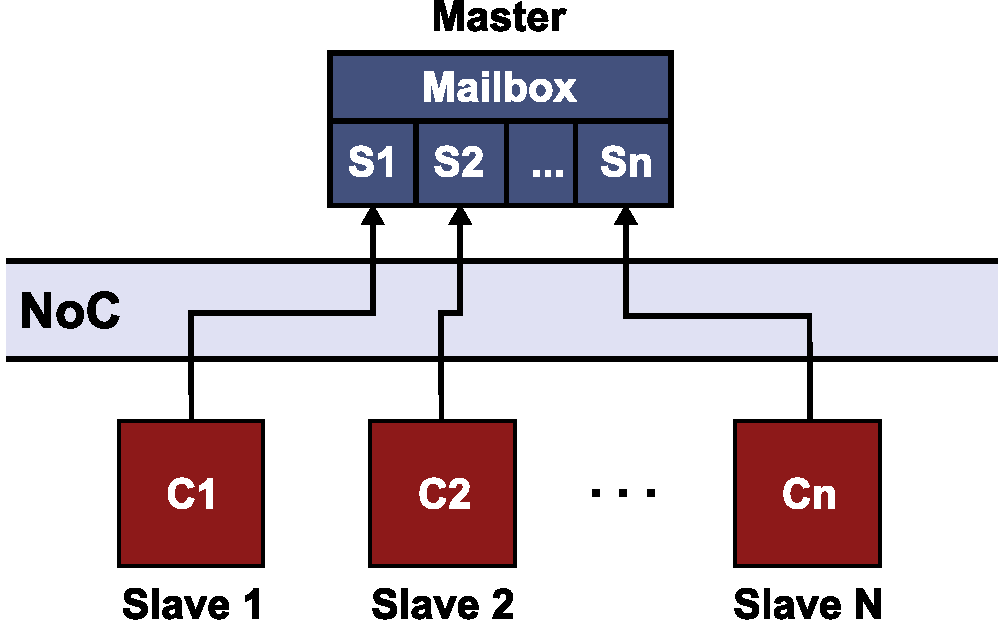
\includegraphics[width=\linewidth]{mailbox-logical.pdf}}%

				\hfill

				\subcaptionminipage[fig:conpt_mailbox-flow]%
					{.6\linewidth}%
					{Flow of execution: Slave sends a message, Master reads and notifies the sender.}%
					{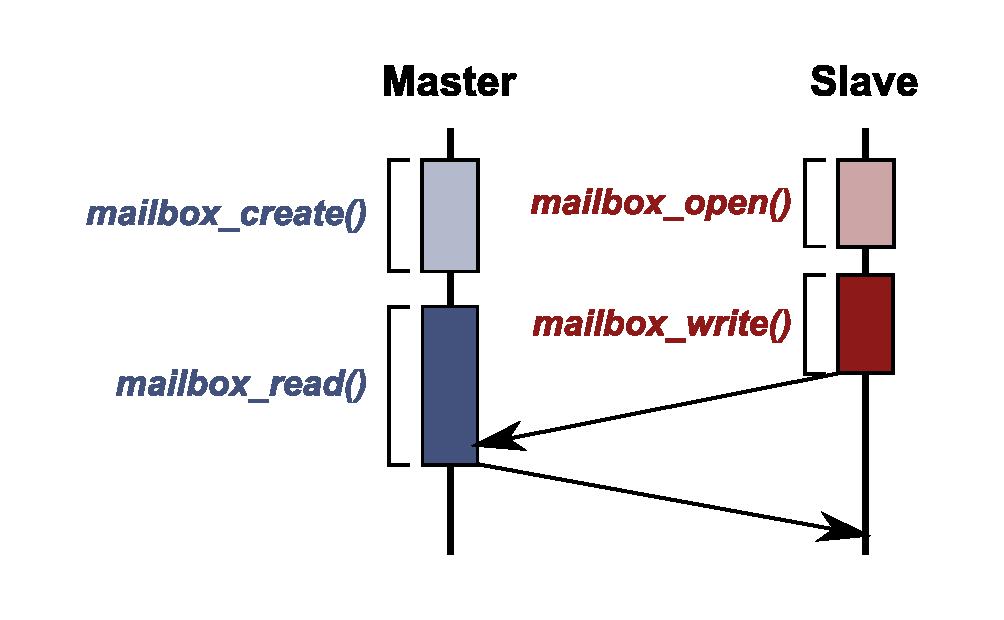
\includegraphics[width=\linewidth]{mailbox-flow.pdf}}%

				\fonte{Developed by the Author.}%
			\end{figure}

			A Figura (fluxo) exemplifica o fluxo de comunicação entre um nó receptor e um emissor.
			A criação de uma Mailbox cria uma fila de mensagens vazia, onde os emissores são livres para enviar a primeira mensagem.
			Posteriormente, todos os envios necessitaram da permissão do receptor para que mensagens não sejam sobreescritas.
			Por este motivo, o receptor notificará o emissor ao consumir sua mensagem.
			A mensagem será copiada para um buffer do usuário e o espaço estará novamente disponível.

			Teoricamente, a quantidade de mensagens permitidas por emissor pode ser de 1 à N.
			Entretanto, optou-se por permitir apenas 1 no Nanvix HAL devido as restrições de memória apresentada por manycores.
			E como o espaço é alocado estatícamente dentro do espaço de memória do kernel, permitir que o usuário escolhe-se o tamanho da fila de mensagem não reduziria o espaço prévio necessário.
			Todavia, o uso de uma mensagem é suficiente para programas servidores tratarem requisitações no nível do Multikernel.
			Por exemplo, a mensagem pode ser usada para codificar pequenas operações e sinais de controle do sistema.

			\subsubsection{Receiver Side Implementation}

				A Mailbox é mais complexa do que o Sync porque utiliza recursos DNoC e CNoC.
				Especificamente, o receptor necessita de 1 slot de recebimento da DNoC e 1 canal de transmissão da CNoC.
				São utilizados dois tamanhos na configuração do slot rx, um para o tamanho de uma mensagem, o qual gerará interrupções, e outro para o tamanho total buffer alocado.
				O buffer é alocado no kernel com espaço suficiente para receber 24 mensagens.
				A mensagem, propriamente dita, é composta por um cabeçalho identificando o emissor, um corpo contendo a mensagem útil e um rodapé com o mesmo identificador.
				O canal de transmissão é utilizado após a cópia da mensagem útil para o buffer do usuário, notificando o ID do cabeçalho.

				O paralelismo no recebimento das mensagens introduziu alguns desafios na leitura assíncrona do Mailbox como 
				(i) cada mensagem gera uma interrupção,
				(ii) interrupções preemptadas por outras não encontraram os recursos da DNoC que emitiram a interrupção e
				(iii) não é possível verificar a quantidade de interrupções geradas por um recurso.
				Para burlar estas barreiras, foi implementado um comportamento similar ao envio preguiçoso.
				Primeiro, um contador global contendo a quantidade total de mensagens recebidas permite que o receptor copie mensagens recebidas antes de uma leitura.
				Segundo, caso não haja mensagens disponíveis, a cópia será realizada pelo próximo disparo do manipulador.
				Terceiro, para resolver o problema das interrupções preemptadas, sempre que um manipulador é disparado ele percorrerá a fila de mensagens conferindo os cabeçalhos e rodapés.
				Ao identificar uma mensagem válida, o manipulador incrementa o contador e altera o rodapé para um código especifico.
				Desta forma, não perdemos nenhuma mensagem por não tratar uma interrupção.

				O código 3 apresenta a interface da Mailbox para um nó receptor.
				A criação de uma Mailbox requer que a aplicação informe o ID Lógico no nó local.
				Esta identificação é necessária por causa do múltiplos nós existentes nos Cluster I/O.
				As demais operações utilizam o identicador retornado na criação da mailbox.
				Para a leitura de uma mensagem, o usuário é obrigado a passar o local onde a mensagem será copiada e o tamanho a ser copiado.
				O tamanho é sempre constante mas é utilizado como verificação da integridade da operação.
				A cópia bem sucedida de uma mensagem liberará o escravo que executar a função de espera.
				Neste processo de liberação, o core mestre executa o flush da mensagem para a SRAM para que o escravo, ao invalidar a sua cache, possa ler a mensagem.

\begin{listing}[!tb]
\caption{Nanvix HAL: Mailbox Interface for Receiver Node.}
\label{code:hal-mailbox-receiver}
\begin{minted}{c}
/* @brief Creates a mailbox. */
int mailbox_create(int nodenum);

/* @brief Destroys a mailbox. */
int mailbox_unlink(int mbxid);

/* @brief Reads data from a mailbox. */
ssize_t mailbox_aread(int mbxid, void * buffer, size_t size);

/**
 * @brief Waits for an asynchronous operation on a
 * mailbox to complete.
 */
int mailbox_wait(int mbxid);
\end{minted}
\fonte{Developed by the Author.}
\end{listing}

			\subsubsection{Sender Side Implementation}

\begin{listing}[!tb]
\caption{Nanvix HAL: Mailbox Interface for Sender Node.}
\label{code:hal-mailbox-sender}
\begin{minted}{c}
/* @brief Opens a mailbox. */
int mailbox_open(int nodenum);

/* @brief Closes a mailbox. */
int mailbox_close(int mbxid);

/* @brief Writes data to a mailbox. */
ssize_t mailbox_awrite(int mbxid, const void * buffer, size_t size);

/**
 * @brief Waits for an asynchronous operation on a
 * mailbox to complete.
 */
int mailbox_wait(int mbxid);
\end{minted}
\fonte{Developed by the Author.}
\end{listing}

					\todo{"On the another hand" does not make sense AGAIN.}
				On the other hand, the sender will allocate a receive signal slot (\texttt{mailbox\_open()})
				before sending its first message to the receiver.
				If the sender attempts to send a message before the receiver has consumed
				the previous message, the sender will be blocked waiting for the sender's notification.
				In this way, flow control is guaranteed, and the sender will not overwrite
				messages unread by the receiver.
				Sending the message will always be executed asynchronously
				because it will always be necessary to copy the message to
				a kernel buffer that contains the header.
				Thus, the sender will never be blocked waiting for the message to be sent.
				In this configuration, the number of mailbox creations (\texttt{mailbox\_create()})
				within a cluster is limited to 1 because of the \cnoc sending channel.
					\todo{"On the another hand" does not make sense AGAIN.}
				On the other hand, the maximum number of opens (\texttt{mailbox\_open()}) is
				4 because of the limitation of the available \dnoc sending channels.

		\subsection{Portal Abstraction}
		\label{sec.portal-abs}

			\begin{figure}[!tb]
				\centering%
				\caption{Portal Abstraction Concept: Node 1 create a portal and notify Node 2 to transfer the data.}%
				\label{fig:conpt_portal}%
				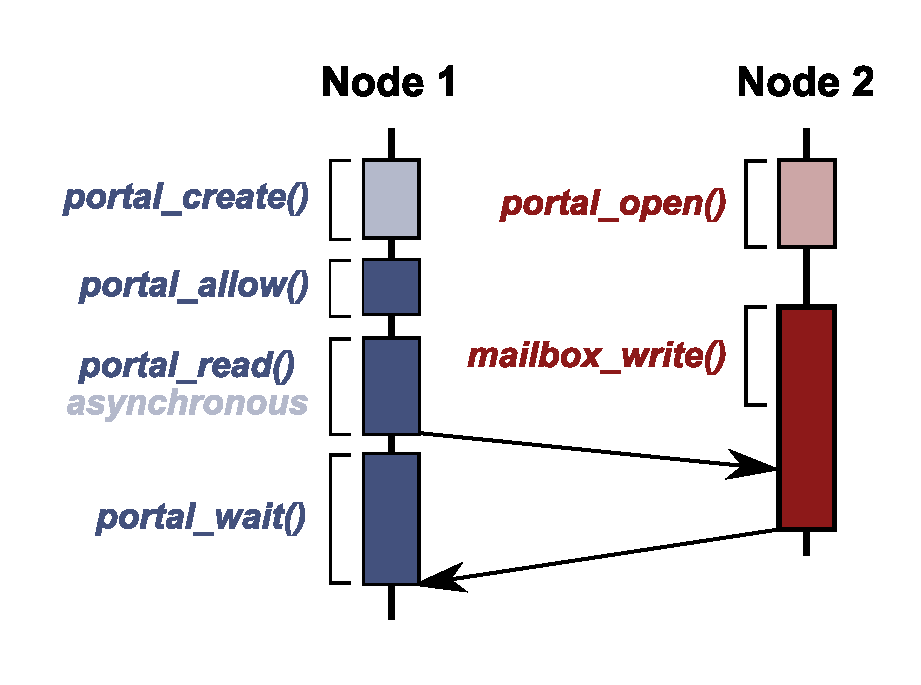
\includegraphics[width=.65\textwidth]{portal.pdf}%
				\fonte{Developed by the Author.}%
			\end{figure}

				\todo[inline]{Make it more detailed.}

			Lastly, the \textit{Portal Abstraction} enables two clusters to exchange arbitrary
			amounts of data.
			The conceptual idea of the \portal is similar to that implemented in \posix pipes.
			\autoref{fig:conpt_portal} shows the \portal operation, with cardinality
			1:1, a cluster pair opens a channel to transfer data.
			However, the operation is only allowed in one direction with a flow control mechanism,
			where the receiver cluster warns the sender cluster when it is ready to receive.

			\subsubsection{Receiver Side Implementation}

\begin{listing}[!tb]
\caption{Nanvix HAL: Portal Interface for Receiver Node.}
\label{code:hal-portal-receiver}
\begin{minted}{c}
/* @brief Creates a portal. */
int portal_create(int local);

/* @brief Destroys a portal. */
int portal_unlink(int portalid);

/* @brief Allow sender to transfer data. */
int portal_allow(int portalid, int remote);

/* @brief Reads data asynchronously from a portal. */
ssize_t portal_aread(int portalid, void * buffer, size_t size);

/**
 * @brief Waits for an asynchronous operation on a
 * portal to complete.
 */
int portal_wait(int portalid);
\end{minted}
\fonte{Developed by the Author.}
\end{listing}

			\subsubsection{Sender Side Implementation}

\begin{listing}[!tb]
\caption{Nanvix HAL: Portal Interface for Sender Node.}
\label{code:hal-portal-sender}
\begin{minted}{c}
/* @brief Opens a portal. */
int portal_open(int remote);

/* @brief Closes a portal. */
int portal_close(int portalid);

/* @brief Writes data asynchronously to a portal. */
int portal_awrite(int portalid, const void * buffer, size_t size);

/**
 * @brief Waits for an asynchronous operation on a
 * portal to complete.
 */
int portal_wait(int portalid);
\end{minted}
\fonte{Developed by the Author.}
\end{listing}

				\autoref{sec.portal-abs} showed that the portal abstraction is similar to
				a \posix pipe with flow control.
				So, the \portal analogously follows the ideas implemented
				in the \mailbox with the difference of the option to write,
				that can be synchronously or asynchronously.
				The total number of receive data operations (\texttt{portal\_create()})
				is limited to 2 because of the number of available signal sending channels.
					\todo{"On the another hand" does not make sense AGAIN.}
				On the other hand, up to 4 send operations (\texttt{portal\_open()})
				can be performed simultaneously because there are 4 available send
				channels for the \portal.

				Function \texttt{portal\_open()} starts the data send operation.
				In it will be allocated a channel of data sending associated with
				a $\mu$thread.
				Also, a signal receiving slot will be allocated to receive the
				signal that will release the sender to transfer data to the receiver.
				In asynchronous send operation (\texttt{portal\_awrite()}), the cluster
				cannot modify or release the buffer until the operation is completed.
				To ensure that the buffer can use, the cluster must call function \texttt{portal\_wait()}.

				The receiver will allocate a receiving slot of the \dnoc and a transfer
				channel (\texttt{portal\_create()}) to receive data from another cluster.
				After setting up the resources (\texttt{portal\_read()}), the receiver
				can notify a sender (\texttt{portal\_allow()}), enabling it to transfer data.
				For this reason, the read operation is always performed asynchronously.
				After receiving the set amount of data, the receiver can use the buffer securely.

	
	\section{User-Level Communication}
	\label{sec.comm-services}
	\todo{Or: Nanvix Microkernel Level}

		\subsection{Inter-Cluster Communication Services}
		\label{sec.inter-cluster-communication-module}

			The inter-cluster communication module, described in \autoref{sec.inter-cluster-communication-module},
			is designed to export a standard and straightforward communication
			primitives to different lightweight manycores.
			These primitives can be used by various types of operating systems
			and applications.
			Thus, the module is flexible enough not to impact the performance
			of the upper layers negatively.
			For this, it does not provide rich management of the exposed abstractions.

			In this scenario, the communication services of Nanvix Microkernel seek
			to provide \ipc between distinct clusters.
			Specifically, these services perform the multiplexing of the hardware
			resources and the verification of the parameters that will be passed
			on the communication primitives.
			Due to the Master-Slave model, the responsibility of protecting,
			manipulating, and configuring \hal resources is of the master core.
			The slave core will request operations through a meta-interface,
			passing the necessary information to the master.

			Considering that the abstractions make up the fundamental elements of
			the construction of more complex services, the Microkernel services
			were responsible for the management and multiplexing of the finite
			resources for the many cores of a cluster.
			In total, there are three communication services in the Nanvix Microkernel,
			each associated with an abstraction of the communication module,
			analogously named \sync, \mailbox, and \portal services.

		\subsection{Inter-Cluster Communication Services Implementation}

			\todo[inline]{Temporary}

			As described in \autoref{sec.communication-services}, three communication
			services will be developed for the Nanvix Microkernel, named \sync, \mailbox,
			and \portal services.
			Each service will be responsible for protecting, managing, manipulating,
			and multiplexing the resources exposed by the \hal communication module.
			These services must take into account the memory constraints and the
			master-slave model chosen for the Microkernel.

			Management and manipulation operations are similar to all services.
			They will be provided through interfaces that function as wrappers
			for the \hal abstraction functions.
			In the implementation of these interfaces, there will be a mapping
			between low-level identifiers, associated with \hal resources,
			and high-level identifiers, associated with resource protection structures.

			\todo[inline]{
				According to Odorico, for the completion of the work, it is important to highlight:
				\\ - How do you treat the protection operations?
				\\ - How do you intend to test and to validate the correctness of the implemented services.
			}

			The protection operations are mostly similar.
			For instance, the use of unallocated resources, sanitizing entries,
			checking valid identifiers, non-null pointers, and checking
			for conflicting operations (reading in write-only resources).
			In the meantime, there are exceptional cases in some services
			that must be taken.
			For instance, in the \sync service, a cluster cannot synchronize
			with itself, or there is a repetition of identifiers in the
			stipulated set of clusters.

			Finally, some aspects of services and implementation still need
			to be analyzed and will be better detailed in another version
			of the dissertation.
			For example, what resource multiplexing methods will be used
			and their impacts on the Nanvix Microkernel services.